\chapter{Latent Model-Based Decision-Aware Actor-Critic}
\label{chap:cvaml}

\newcommand{\rev}[1]{#1}

\section{Introduction}
In model-based reinforcement learning, an agent collects information in an environment and uses it to learn a model of the world to accelerate and improve value estimation or the agent's policy~\parencite{dyna,deisenroth2011pilco, Hafner2020Dream,schrittwieser2020mastering}.
However, as environment complexity increases, learning a model becomes more and more challenging. 
These model errors can impact the learned policy~\parencite{schneider1997exploiting,kearns2002near,talvitie2017self,lambert202objective} leading to worse performance.
In many realistic scenarios, agents are faced with a "big world" where learning to accurately simulate the environment is infeasible.
When faced with complex environments, deciding what aspects of the environment to model is crucial.
Otherwise, capacity would be spent on irrelevant aspects, e.g., modelling clouds in a vehicle's video feed.

Recently, the paradigm of \emph{decision-aware model learning} (DAML)~\parencite{vaml} or \emph{value equivalence}~\parencite{grimm2020value,grimm2021proper} has been proposed.
The core idea is that a model should make predictions that result in correct value estimation.
Two prominent algorithms in the space of decision-aware model learning are the IterVAML~\parencite{itervaml} and MuZero~\parencite{schrittwieser2020mastering} algorithms.
While IterVAML is a theoretically grounded algorithm, difficulties in adapting the loss for empirical implementations have been highlighted in the literature~\parencite{lovatto2020decision,voelcker2022value}.
MuZero on the other hand has been shown to perform well in discrete control tasks~\parencite{schrittwieser2020mastering,ye2021mastering} but has received little theoretical investigation. Thus, understanding the role of different value-aware losses and determining the factors for achieving strong performance is an open research problem.

In this work, we address this problem by establishing similarities and differences between these two approaches. 
Our goal is to establish an algorithmic framework and to provide insight into the strengths and weaknesses of each.
Experimental evaluations focus on the state-based DMC environments \parencite{tunyasuvunakool2020}, as the focus of our paper is not to scale up to image-based observations.

The main differences between previous works trying to build on the IterVAML and MuZero algorithms are neural network architecture design \rev{and the value function learning scheme}.
MuZero is built on value prediction networks \parencite{oh2017value}, which explicitly incorporate a latent world model, while IterVAML is designed for arbitrary model choices.
We show that the use of latent models can explain many previously reported performance differences between MuZero and IterVAML \parencite{voelcker2022value,lovatto2020decision}.

As a theoretical contribution, we prove a conjecture by \textcite{oh2017value} that IterVAML and MuZero-based models can achieve low error in stochastic environments, even when using deterministic world models.
To the best of our knowledge, we are the first to prove the conjecture.
The MuZero \rev{value function learning scheme} however results in a bias in stochastic environments.
We show that this bias leads to a quantifiable difference in performance.
\rev{Finally, we show that the model learning component of MuZero is similar to VAML, which was previously also noted by \textcite{grimm2021proper}}.

Finally, we show when decision-aware losses provide benefits in practice and propose new ways to combine them with policy gradient estimation approaches.
To highlight that many design decisions can be combined freely with one another, we propose to treat previous approaches as parts of a family of algorithms, which we call Latent Model-Based Decision-Aware Actor-Critic ($\lambda$-AC) methods.
$\lambda$-AC algorithms combine three core components: a latent world model, a value-aware model loss function, and a model-based actor-critic algorithm for reinforcement learning.

In summary, our contributions are a) showing that IterVAML is a stable loss when a latent model is used, b) proving and verifying that the MuZero value loss is biased in stochastic environments, and c) showing how novel combinations of established algorithms provide benefits in benchmarks.

\section{Background}
We consider a standard Markov decision process (MDP)~\parencite{Puterman1994MarkovDP,suttonbook} $(\mathcal{X}, \mathcal{A}, p, r, \gamma)$, with state space $\mathcal{X}$, action space $\mathcal{A}$, transition kernel $p(x'|x,a)$, reward function $r: \mathcal{X} \times \mathcal{A} \xrightarrow[]{} \mathbb{R}$, and discount factor $\gamma \in [0,1)$.
The goal of an agent is to optimize the obtained average discounted infinite horizon reward under its policy: $\max_\pi \mathbb{E}_{\pi,p}\squareb{\sum_{t=0}^{\infty} \gamma^t r(x_t, a_t)}$.

Given a policy $\pi(a|x)$, the value function is defined as the expected return conditioned on a starting state $x$: $V^\pi(x) = \EEX{\pi}{\sum_{t \geq 0} \gamma^t r_t|x_0 = x}$, where $r_t = r(x_t, a_t)$ is the reward at time $t$.
The value function is the unique stationary point of the \emph{Bellman operator} $\mathcal{T}_p(V)(x) = \EEX{\pi(a|s)}{r(x,a) + \gamma  \EEX{p(x'|x,a)}{V(x')}}$.
The action-value function is defined similarly as $Q^\pi(x,a) = \EEX{\pi}{\sum_{t \geq 0} \gamma^t r_t|x_0 = x, a_0 = a}$.
In this work, we do not assume access to the reward functions and denote learned approximation as $\hat{r}(x,a)$.

An \emph{environment model} is a function that approximates the behavior of the transition kernel of the ground-truth MDP.\footnote{In this paper, we will generally use the term \emph{model} to refer to an environment model, not to a neural network, to keep consistent with the reinforcement learning nomenclature.}
Learned models are used to augment the reinforcement learning process in several ways~\parencite{dyna,mbpo,Hafner2020Dream}, we focus on the MVE \parencite{buckman2018sample} and SVG \parencite{amos2021model} algorithms presented in details in \autoref{sec:ac}.

We will use $\hat{p}(x'|x,a)$ to refer to approximate model, and use $\hat{f}(x,a)$ when referring specifically to deterministic models.
All models which take a state $x\in\mathcal{X}$ as an input and map to distributions over $\mathcal{X}$ will be referred to as \emph{observation-space models}.
An alternative are \emph{latent models} of the form $\hat{p}(z'|z, a)$, where $z\in\mathcal{Z}$ is a representation of a state $x\in\mathcal{X}$ given by $\phi: \mathcal{X} \rightarrow \mathcal{Z}$.
Analogously, latent deterministic models are also possible $\hat{f}: \mathcal{Z} \times \mathcal{A} \rightarrow \mathcal{Z}$.
In the following, the difference will be clear from context.
We present further details on latent model learning in \autoref{sec:representations}.

The notation $\hat{x}^{(n)}_{i}$ refers to an $n$-step rollout obtained from a model by starting in state $x_{i}$ and sampling the model for $n$-steps.
We will use $\hat{p}^n\roundb{x^{(n)}\middle|x}$ and $\hat{f}^n(x)$ to refer to the $n$-th step model prediction.

\subsection{Decision-Aware Model Losses}
\label{sec:model_losses}

\begin{figure}[t]
    \centering
    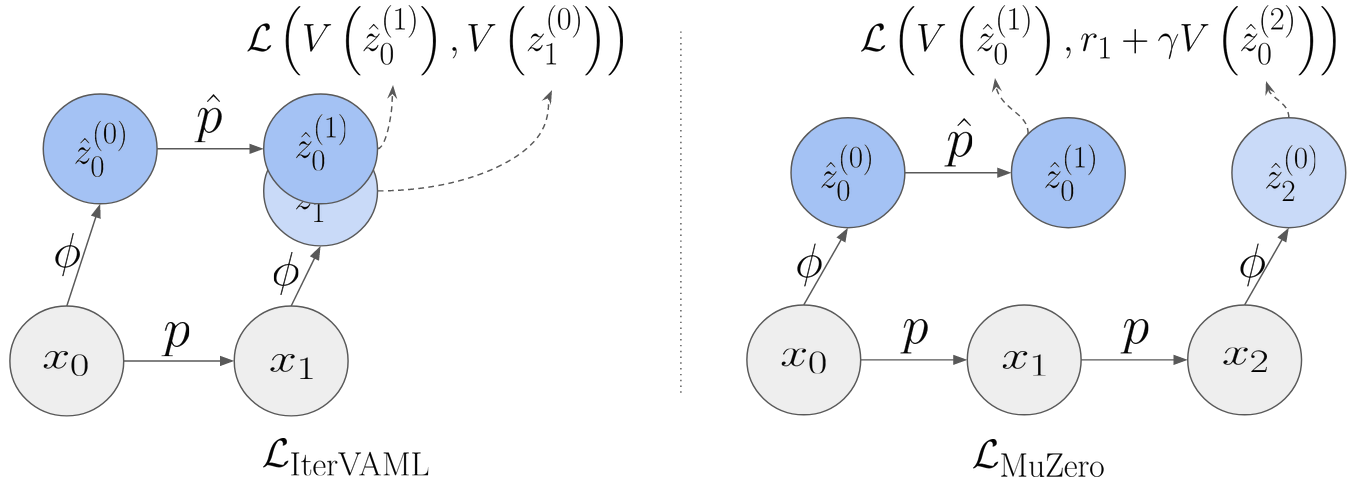
\includegraphics[width=.8\textwidth]{illustrations/lambda/loss_comparison_names.png}
    \caption{Sketch of the different value-aware losses with latent models. IterVAML computes the value function difference between the latent prediction and the next state encoding, while MuZero computes a single-step bootstrap estimate.}
    \label{fig:loss_graphic}
\end{figure}

The losses of the decision-aware learning framework share the goal of finding models that provide good value function estimates.
Instead of simply learning a model using maximum likelihood estimation, the value function is directly used in the model update. 

Given a distribution $\mu$ over the state space and a value function approximation $\hat{V}$, the IterVAML loss~\parencite{itervaml} is defined as
\begin{align}
    \mathcal{L}_\text{IterVAML}(\hat{p}; \mu, \hat{V}, p) = \EEX{x, a \sim \mu}{\abs{\int_\mathcal{X} \roundb{\hat{p}(x'|x, a) - p(x'|x, a)} \hat{V}(x') \mathrm{d}x'}^2}.\label{eq:itervaml}
\end{align}

Although not originally presented by \cite{itervaml}, this formulation can be easily extended to a multi-step version $\mathcal{L}^n_\text{IterVAML}$\footnote{A more detailed discussion of this extension is found in \autoref{app:multi-step-itervaml}}.
In practice, we assume access to a dataset of state and reward sequences $\mathcal{D} = \{x_{i_1}, r_{i_1}, \dots, x_{i_n}, r_{i_n}\}_{i=1}^N$ with $x_{i_1}$ sampled from $\mu$ and subsequent states sampled according to the transition function.
Note that the index $1$ here denotes the start of a sequence, not the start of an episode, and sequences can be overlapping. 
% This is similar to other losses in related works~\parencite{Hafner2020Dream,amos2021model,ghugare2023simplifying}.
Then, the sample-based IterVAML loss is \
\begin{align}
    \hat{\mathcal{L}}^n_\text{IterVAML}(\hat{p}; \hat{V}, \mathcal{D}) &= \frac{1}{N\cdot n}\sum_{i=1}^N \sum_{j=1}^n \squareb{\EEX{\hat{x}^{(j)}\sim \hat{p}^j(\cdot|x_{i_1}, a_{i_1})}{\hat{V}\roundb{\hat{x}^{(j)}}} - \hat{V}\roundb{x_{i_j}} }^2.
\end{align}

The population-based MuZero loss is not defined in the literature, but the sample-based version is.
Similar to \textcite{dqn}, it uses a target network for the value function, which we denote as $V_\text{target}$. The MuZero loss is given as 
\begin{align}
    \hat{\mathcal{L}}^n_\text{MuZero}\left(\hat{f}, \hat{V}; \mathcal{D}, V_\text{target}\right) &= \frac{1}{N\cdot n}\sum_{i=1}^N \sum_{j=i}^n \squareb{ \hat{V}\roundb{\hat{f}^j(x_{i_1}, a_{i_1})} - \squareb{r_{i_j} + \gamma V_\text{target}\roundb{x_{i_{j+1}}} }}^2. \label{eq:muzero}
\end{align}

Note that the real environment reward and next states are used in the $j$-th step.
The main difference between the two loss formulations is that IterVAML uses a squared minimization between two value function outputs, while MuZero computes the value function target via bootstrap.
For the $1$-step case, this is illustrated in \autoref{fig:loss_graphic}.
The MuZero loss is also used for updating both the value function and the model, while IterVAML is only designed to update the model and uses a model-based bootstrap target to update the value function.

Decision-aware losses can be insufficient for sample-efficient learning ~\parencite{ye2021mastering}, especially in continuous state-action spaces~\parencite{tdmpc}.
Their performance is improved greatly by using an auxiliary latent self-prediction loss based on the \emph{Bootstrap your own latent} (BYOL) loss~\parencite{grill2020bootstrap}.
Several different versions of this loss have been proposed for RL~\parencite{gelada2019deepmdp,schwarzer2021dataefficient,tang2022understanding}, we consider a simple $n$-step variant:
\begin{align}
    \hat{\mathcal{L}}^n_\text{latent}\roundb{\hat{f}, \phi; \mathcal{D}} = \frac{1}{N\cdot n}\sum_{i=1}^N \sum_{j=1}^n \squareb{\hat{f}^{(j)}(\phi(x_{i_1}), a_{i_1}) - \text{stop-grad}\squareb{\phi(x_{i_j})}}^2.
\end{align}
Theoretical analysis of this loss by \textcite{gelada2019deepmdp} and \textcite{tang2022understanding} also shows that the learned representations provide a good basis for value function learning.

\subsection{Actor-critic learning}
\label{sec:ac}

Both IterVAML and MuZero can use the model to approximate the value function target. 
In its original formulation, MuZero is used with a Monte Carlo Tree Search procedure to expand the model which is not directly applicable in continuous state spaces.
A simple alternative for obtaining a value function estimate from the model in continuous state spaces is known as model value expansion (MVE)~\parencite{feinberg2018model}.
In MVE, short horizon roll-outs of model predictions $[{\hat{x}^{0},\dots,\hat{x}^{n}}]$ are computed using the current policy estimate, with a real sample from the environment as a starting point $x^{(0)}$.
Using these, \textit{n}-step value function targets are computed
% In our experiments, we use a standard twinned delayed target network $\bar{Q}$ to reduce overestimation in the value function estimate.
    $Q_\text{target}^j\roundb{\hat{x}^{(j)},\pi\roundb{\hat{x}^{(j)}}} = \sum_{i=j}^{n-1} \gamma^{i-j} \hat{r}\roundb{\hat{x}^{(i+j)}, \pi\roundb{\hat{x}^{(i+j)}}} + \gamma^{n-j} \bar{Q}\left(\hat{x}^{(n)}, \pi\roundb{\hat{x}^{(n)}}\right) \label{eq:mve_target}$.
These targets represent a bootstrap estimate of the value function starting from the \textit{j}-th step of the model rollout.
For our IterVAML experiments, we used these targets together with TD3 \parencite{td3} to learn the value function, for MuZero, we used these targets for $V_\text{target}$ in \autoref{eq:muzero}.

%The $j$-step formulation ensures that intermediate value functions at states which only appear in the model rollout are also updated based on the approximate value function of the model predictions.
% Note that the value function gradient is not used to update the model and the bootstrap is computed using the model, two core differences between this approach and the MuZero algorithm outlined above.


In continuous control tasks, estimating a policy is a crucial step for effective learning algorithms.
To improve policy gradient estimation with a model, model-based value gradients~\parencite{heess2015learning,amos2021model} can be used.
Model-based policy gradients~\parencite{heess2015learning} are obtained by differentiating the full \textit{n}-step MVE target (\autoref{eq:mve_target}) with regard to the policy.
If differentiable policies and models are used, a policy gradient over the complete computational graph of the model rollout is obtained.
% In the case of stochastic environments or stochastic policies, this approach only provides a biased approximation of the true policy gradient~\parencite{lovatto2021gradient}.
% However differentiating the model greatly reduces the variance of the policy gradient estimates and is therefore useful nonetheless.
We evaluate the usefulness of model-based policy gradients in \autoref{sec:experiments_mve}, with deterministic policy gradients~\parencite{silver2014deterministic,ddpg} as a model-free baseline.

\section{Latent Decision Aware Models}
\label{sec:lambda-intro}

\begin{wrapfigure}[28]{r}{0.37\textwidth}
    \centering
    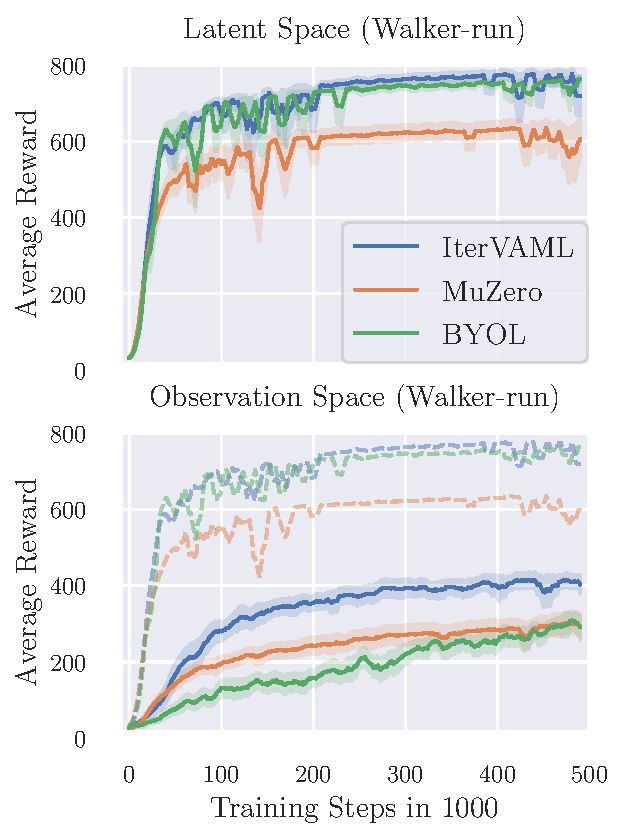
\includegraphics[width=.35\textwidth]{figures/lambda/latent_2.pdf}
    \caption{Comparison on the use of an explicit latent space with different loss functions. All losses improve in performance from the addition of an explicit latent space transformation. Dashed lines represent the mean of the latent space result. The experiments are repeated over eight random seeds and shaded areas mark three $\sigma$ of the standard error of the mean over seeds.}
    \label{fig:latent}
\end{wrapfigure}

To compare previous work in decision-aware MBRL \parencite{vaml,itervaml,schrittwieser2020mastering,grimm2021proper}, we propose to view both MuZero and IterVAML as members of a family of algorithms, which we call \emph{Latent Decision Aware Model Based Actor Critic} framework ($\lambda$-AC) for convenience.
A $\lambda$-AC algorithm is composed of three primary components: a latent model learning architecture, a decision aware model learning loss, and an actor-critic algorithm to obtain a control policy.\footnote{For an overview of the differences and similarities of different value aware loss, see \autoref{app:lambda-table}.}


In this work, we consider the MuZero and IterVAML model learning losses, with the MuZero value function learning scheme and model-based bootstrap.
We are interested in understanding what components of the algorithms lead to performance differences in practice.
To clarify the nomenclature, we designate the combination of the MuZero model and value function learning algorithm combined with the SVG objective as $\lambda$-MuZero, and the combination of IterVAML, model-based MVE and SVG as $\lambda$-IterVAML.

\subsection{The importance of latent spaces for applied decision-aware model learning} \label{sec:representations}


One of the major differences between MuZero and IterVAML is that the former uses a latent model design, while the IterVAML algorithm is presented without a specific architecture.
When used with a state-space prediction model, IterVAML has been shown to diverge, leading to several works claiming that it is an impractical algorithm~\parencite{lovatto2020decision,voelcker2022value}.
However, there is no a priori reason why a latent model should not be used with IterVAML, or why MuZero has to be used with one.
In prior work, sharp value function gradients have been hypothesized to be a major concern for IterVAML~\parencite{voelcker2022value}.
The introduction of a learned representation space in the model through a latent embedding can help to alleviate this issue.

The full loss for each experiment is $\mathcal{L}^n_\text{DecisionAware} + \mathcal{L}^n_\text{latent} + \mathcal{L}^n_\text{reward}$, where $\mathcal{L}_\text{reward}$ is an MSE term between the predicted and ground truth rewards.
As a baseline, we drop the decision-aware loss and simply consider BYOL.
Full pseudocode is found in \autoref{app:pseudocode}.
As is evident from \autoref{fig:latent} the latent space is highly beneficial to achieve good performance.
For all of our experiments we use eight random seeds and the shaded areas mark three $\sigma$ of the standard error of the mean over random seeds, which represents a $99.7\%$ certainty interval under a Gaussian assumption.


This highlights that negative results on the efficacy of IterVAML are largely due to suboptimal choices in the model implementation, not due to limitations of the algorithm.
In addition, the stabilizing loss is essential for IterVAML, while it can be dropped in MuZero~\parencite{ye2021mastering} (compare \autoref{app:more_experiments}).
We conjecture that MuZero is more stable without auxiliary losses due to incorporating the true reward into its joint model-value function loss, an advantage that IterVAML does not have.
The weak performance of MuZero on walker-run sepcifically seems to be an outlier, compare \autoref{sec:experiments}.


\section{Analysis of decision-aware losses in stochastic environments}
\label{sec:theory}

While the two losses behave similarly in deterministic environments, it is an open question if this holds in stochastic ones.
While previous work has noted deterministic models to be insufficient in stochastic cases~\parencite{antonoglou2022planning}, we presented a theoretical treatment and an analysis of the loss functions of both MuZero and IterVAML.
Proofs are found in \autoref{app:main_proofs}.

In Proposition \ref{prop:1} we establish that $\lambda$-IterVAML leads to an unbiased solution in the infinite sample limit, even when restricting the model class to deterministic functions under measure-theoretic conditions on the function class.
This is a unique advantage of value-aware models.
Algorithms such as Dreamer~\parencite{Hafner2020Dream} or MBPO~\parencite{mbpo} require stochastic models.


We then show in Proposition \ref{prop:2} that MuZero's joint model- and value function learning algorithm leads to a biased solution, even when choosing a probabilistic model class that contains the ground-truth environment.
This highlights that while the losses are similar in deterministic environments, the same does not hold in the stochastic case.
Finally, we verify the theoretical results empirically by presenting stochastic extensions of environments from the DMC suite \parencite{tunyasuvunakool2020}.

\subsection{Restricting IterVAML to deterministic models}


In most cases, deterministic function approximations cannot capture the transition distribution on stochastic environments.
However, it is an open question whether a deterministic model is sufficient for learning a \emph{value-equivalent} model, as conjectured by \parencite{oh2017value}.
We answer this now in the affirmative.
Showing the existence of such a model relies on the continuity of the transition kernel and involved functions $\phi$ and $V$.\footnote{To reduce notational complexity, we ignore the action dependence in all following propositions; all results hold without loss of generality for the action-conditioned case as well.}

\begin{proposition}
\label{prop:1}
    Let $\mathcal{X}$ be a compact, connected, metrizable space. Let $p$ be a continuous kernel from $\mathcal{X}$ to probability measures over $\mathcal{X}$. Let $\mathcal{Z}$ be a metrizable space. Consider a bijective latent mapping $\phi: \mathcal{X} \rightarrow \mathcal{Z}$ and any $V: \mathcal{Z} \rightarrow \mathbb{R}$. Assume that they are both continuous. Denote $V_\mathcal{X} = V \circ \phi$.
    
    Then there exists a measurable function $f^*: \mathcal{Z} \rightarrow \mathcal{Z}$ such that we have $V(f^*(\phi(x))) = \EEX{p}{V_\mathcal{X}(x')|x}$ for all $x \in \mathcal{X}$.
\end{proposition}

We can conclude that given a sufficiently flexible function class $\mathcal{F}$, IterVAML can recover an optimal deterministic model for value function prediction.
Note that our conditions solely ensure the \emph{existence} of a measurable function; the learning problem might still be very challenging.
Nonetheless, even without the assumption that the perfect model $f$ is learnable, the IterVAML loss finds the function that is closest to it in the mean squared error sense, as shown by \textcite{itervaml}.

\subsection{Sample bias of MuZero' value function learning algorithm}
\label{sec:muzero_bias}


MuZero is a sound algorithm for deterministic environments, however, the same is not true for stochastic ones.
While changed model architecture for MuZero have been proposed for stochastic cases~\parencite{antonoglou2022planning}, the value function learning component contains its own bias.
% While the rest of the paper focuses on continuous state-spaces, this result also holds for discrete state-spaces.
To highlight that the problem is neither due to the $n$-step formulation nor due to suboptimal architecture or value function class, we show that the value function estimate does not converge to the model Bellman target using the MuZero loss.
Intuitively, the problem results from the fact that two samples drawn from the model and from the environment do not coincide, even when the true model and the learned model are equal (see \autoref{fig:muzero_bias}).
This bias is similar to the double sampling issue in Bellman residual minimization, but is distinct as the introduction of the stop-gradient in MuZero's loss function does not address the problem.


\begin{wrapfigure}[16]{r}{0.27\textwidth}
  \begin{center}
    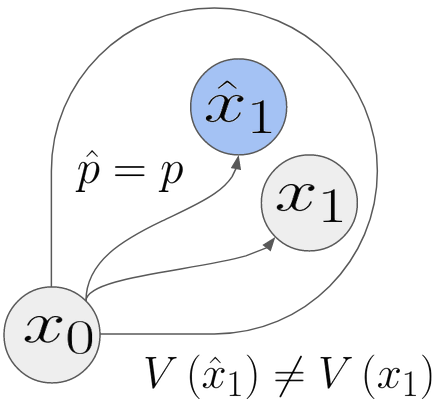
\includegraphics[width=0.25\textwidth]{illustrations/lambda/muzero_bias.png}
  \end{center}
  \caption{The source of the MuZero bias. Though $x_1$ and $\hat{x}_1$ are drawn from the same distribution, their values do not coincide.}
  \label{fig:muzero_bias}
\end{wrapfigure}


\begin{proposition}
\label{prop:2}
    Assume a non-deterministic MDP with a fixed, but arbitrary policy $\pi$, and let $p$ be the transition kernel. 
    % Assume that the MDP and $\pi$ are such that the value function $V^\pi$ is not constant almost everywhere.
    % Let $\mathcal{D}$ be a dataset of tuples $\{s,a,r,s'\}$ collected from a distribution that covers the state-action space fully. 
    Let $\mathcal{V}$ be an open set of functions, and assume that it is Bellman complete: $\forall V \in \mathcal{V}: \mathcal{T}V \in \mathcal{V}$.
    
    \rev{Then for any $V' \in \mathcal{V}$ that is not a constant function, $ \mathcal{T}V' \notin \argmin_{\hat{V} \in \mathcal{V}} \mathbb{E}_{\mathcal{D}}\squareb{\hat{\mathcal{L}}_\text{MuZero}^1(p, \hat{V}; \mathcal{D}, V')}$.}
\end{proposition}

The bias indicates that MuZero will not recover the correct value function in environments with stochastic transitions, even when the correct model is used and the function class is Bellman complete.
On the other hand, model-based MVE such as used in $\lambda$-IterVAML can recover the model's value function in stochastic environments.

The bias is dependent on the variance of the value function with regard to the transition distributions.
This means that in some stochastic environments the MuZero loss might still perform well.
But as the variance of the value function increases, the bias to impact the solution.

If the MuZero loss is solely used for model learning and the value function is learned fully model-free or model-based, the IterVAML and MuZero algorithms show strong similarities (compare \autoref{app:comp_itervaml_muzero}). 
The main difference is that MuZero uses a bootstrap estimate for the value function, while IterVAML uses the value function estimate directly.
However, when jointly training value function and model in a stochastic environment, neither the model nor the value function converge to the correct solution, due to the tied updates.
% This means that the MuZero loss can also learn a deterministic model in stochastic cases, as conjectured in \parencite{oh2017value}, but only when applied to model learning alone.


\subsection{Empirical validation of the performance in stochastic environments}

\begin{figure}[b]
    \centering
    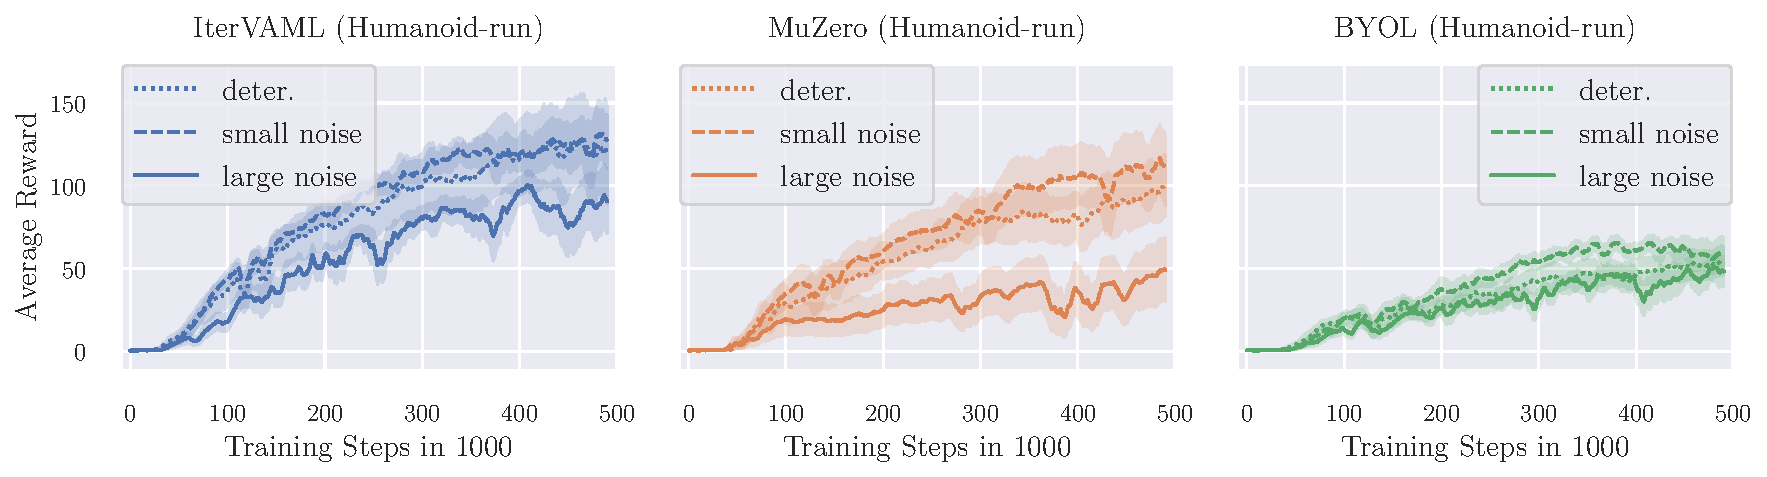
\includegraphics[width=\textwidth]{figures/lambda/noise.pdf}
    \caption{Comparison of the impact of noise across all algorithms. While both IterVAML and MuZero are impacted by the level of noise, we observe a larger drop in MuZero, which does not perform above the BYOL baseline at the highest noise level.}
    \label{fig:noise}
\end{figure}

To showcase that the bias of MuZero's value learning strategy is not merely a mathematical curiosity, we tested the two losses in the challenging humanoid-run tasks from the DMC benchmarking suite~\parencite{tunyasuvunakool2020} with different noise distributions applied to the action (details on the environment can be found in \autoref{app:model_design}).


As shown in \autoref{fig:noise}, we do see a clear difference between the performance of $\lambda$-IterVAML and $\lambda$-MuZero when increasing the noise level.
At small levels of noise, all algorithms retain their performance.
This is expected, since small noise on the actions can increase the robustness of a learned policy or improve exploration \parencite{hollenstein2022action}.
At large levels of noise, however, the $\lambda$-MuZero algorithm drops in performance to the value-unaware baseline.
We provide additional experiments with more stochastic environments in \autoref{app:more_experiments} which further substantiate our claims.

\begin{figure}[b]
    \centering
    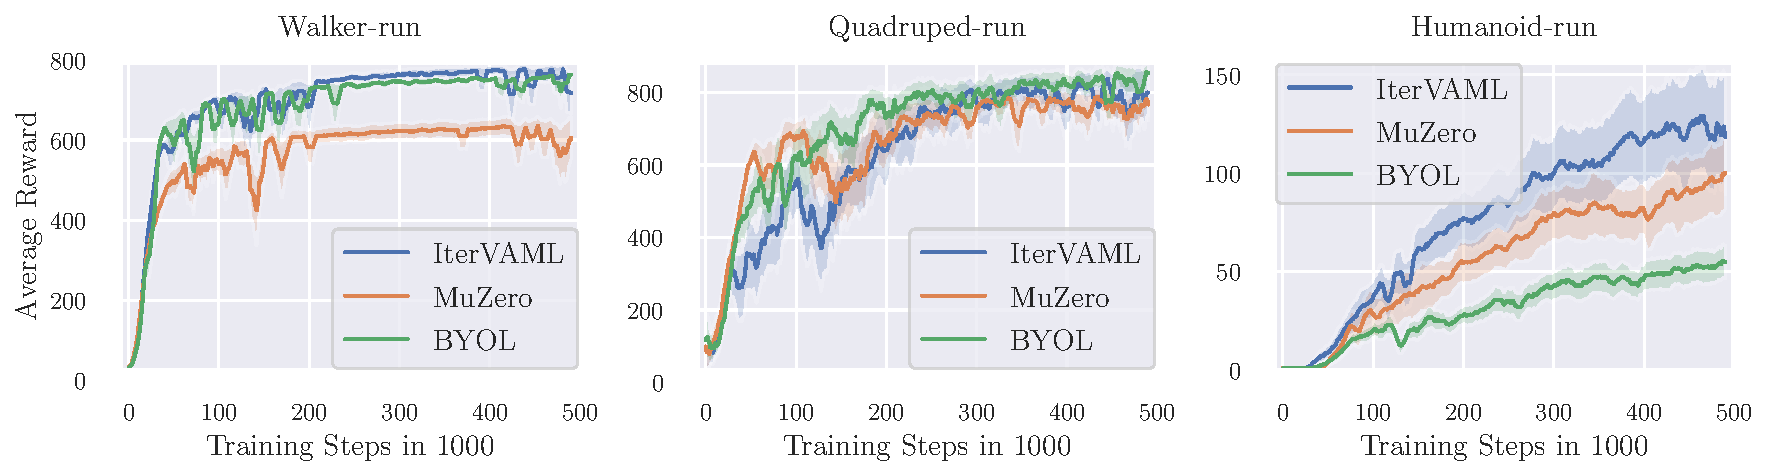
\includegraphics[width=\textwidth]{figures/lambda/full.pdf}
    \caption{Performance comparison overall test environments. We see that IterVAML performs slightly above MuZero in several environments, but decisive gains from the value-aware losses ($\lambda$-IterVAML, $\lambda$-MuZero) over BYOL can only be observed in the challenging Humanoid-run environment.}
    \label{fig:full}
\end{figure}

It is important to note that humanoid-run is a challenging environment and strong noise corruption increases difficulty, therefore $\lambda$-IterVAML will not retain the full performance in the stochastic version.
Furthermore, as highlighted before, the stabilizing latent prediction loss is necessary for $\lambda$-IterVAML and introduces some level of bias (for details see \autoref{app:bias_latent_model}).
However, as all algorithms are impacted by the stabilization term, it is still noticeable that $\lambda$-MuZero's performance drops more sharply.
This raises an important direction for future work, establishing a mechanism for stabilizing value-aware losses that does not introduce bias in stochastic environments.

\section{Evaluating model capacity and environment choice}
\label{sec:experiments}

After investigating the impact of action noise on different loss function, we now present empirical experiments to further investigate how different implementations of $\lambda$-AC behave in empirical settings.
Theoretical results~\parencite{vaml,itervaml} show that value-aware losses perform best when learning a correct model is impossible due to access to finite samples or model capacity.
Even though the expressivity of neural networks has increased in recent years, we argue that such scenarios are still highly relevant in practice.
Establishing the necessary size of a model a priori is often impossible, since RL is deployed in scenarios where the complexity of a solution is unclear.
Increasing model capacity often comes at greatly increased cost~\parencite{kaplan2020scaling}, which makes more efficient alternatives desirable.
Therefore, we empirically verify under what conditions decision-aware losses show performance improvements over the simple BYOL loss.

To replace the MCTS based policy in discrete state-space MuZero, we introduced the use of model value gradients with decision-aware losses.
However, all loss functions were originally designed only for improving value function estimation.
We verify that they still provide benefit for policy gradient approximation by replacing the model-based policy gradient with a model-free version.

For these experiments, we use environments from the popular DMC suite~\parencite{tunyasuvunakool2020}, Walker-run, Quadruped-run, and Humanoid-run.
These environments were picked from three different levels of difficulty~\parencite{tdmpc} and represent different challenge levels in the benchmark, with Humanoid-run being a serious challenge for most established algorithms.

The algorithmic framework and all model design choices are summarized in \autoref{app:model_design}.
The model implementation follows \textcite{tdmpc}. 
Reported rewards are collected during training, not in an evaluation step, the same protocol used by \textcite{tdmpc}.


\paragraph{When do decision-aware losses show performance improvements over the simple BYOL loss?}
The results in \autoref{fig:full} show that both MuZero and IterVAML provide a benefit over the BYOL loss in the most challenging environment, Humanoid-run.
This is expected, as modelling the full state space of Humanoid-run is difficult with the model architectures we used.
For smaller networks, we see a stable performance benefit in \autoref{fig:small} from the MuZero loss.
$\lambda$-IterVAML also outperforms the BYOL baseline, but fails to achieve stable returns.

\begin{wrapfigure}[26]{r}{.37\textwidth}
    \centering
    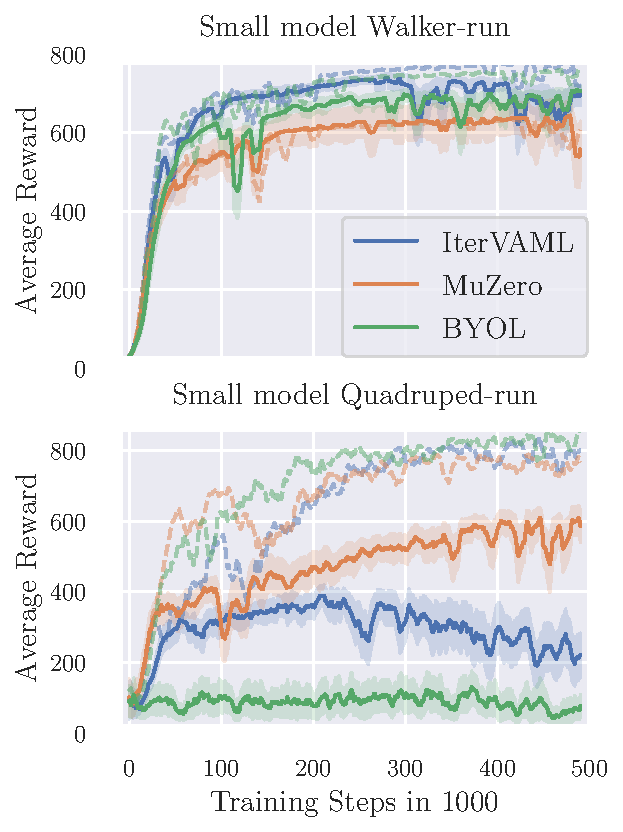
\includegraphics[width=.35\textwidth]{figures/lambda/small_2.pdf}
    \caption{Comparison with smaller models. IterVAML is more impacted by decreasing model size on more challenging tasks, due to the lack of real reward signal in the value function loss. Humanoid is omitted as no loss outperforms a random baseline. Dashed lines show the mean results of the bigger models for comparison.}
    \label{fig:small}
\end{wrapfigure}

This highlights that in common benchmark environments and with established architectures, value-aware losses are useful in challenging, high-dimensional environments.
However, it is important to note that we do not find that the IterVAML or MuZero losses are harmful in deterministic environments, meaning a value-aware loss is always preferable.


The performance improvement of MuZero over IterVAML with very small models is likely due to the effect of using real rewards for the value function target estimation.
In cases where the reward prediction has errors, this can lead to better performance over purely model-based value functions such as those used by IterVAML.

\paragraph{Can decision-aware models be used for both value function learning and policy improvement?}
\label{sec:experiments_mve}

\begin{figure}[b]
    \centering
    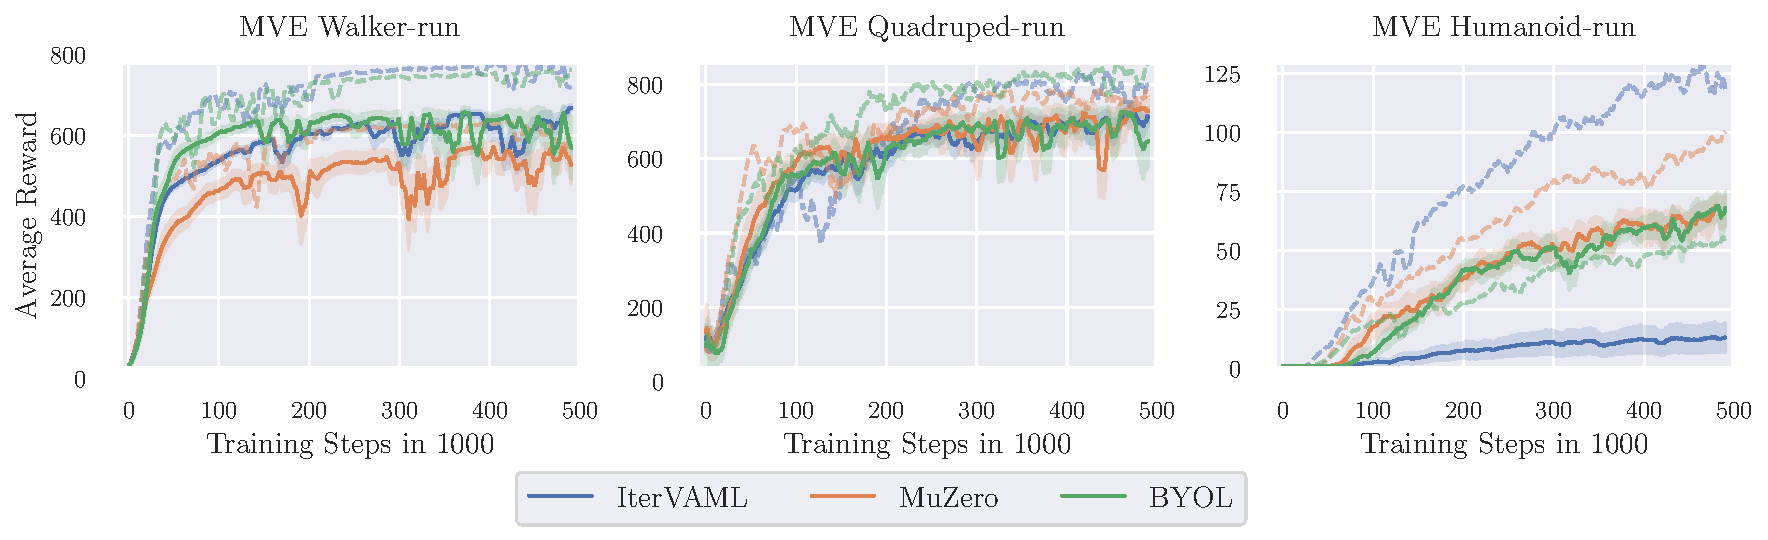
\includegraphics[width=\textwidth]{figures/lambda/mve_b_legend.pdf}
    \caption{Comparison of the impact removing model policy gradients in all environments. Overall we see decreases in performance across all environments and loss functions, with a drastic decrease in performance for IterVAML in the hardest task. Dashed lines show the mean results of the model-based gradient for comparison.}
    \label{fig:mve}
\end{figure}

In all previous experiments, the models were used for both value function target estimation and for policy learning with a model-based gradient.
To investigate the performance gain from using the model for policy gradient estimation, we present an ablation on all environments by substituting the model gradient with a simple deep deterministic policy gradient.

As seen in \autoref{fig:mve}, all losses and environments benefit from better policy estimation using the model.
Therefore it is advisable to use a $\lambda$-AC model both for gradient estimation and value function improvement.
Compared to MuZero, IterVAML loses more performance without policy gradient computation in the hardest evaluation task.
It has been noted that model-based value function estimates might be more useful for policy gradient estimation than for value function learning~\parencite{amos2021model,ghugare2023simplifying}.
In addition, the grounding of the MuZero loss in real rewards leads to better value function prediction in the Humanoid-run environment.
Therefore a better gradient can be obtained with MuZero when the model is not used for policy gradient estimation, since a correct value function estimate becomes more important.

\section{Related work}

\paragraph{VAML and MuZero} \textcite{itervaml}  established the IterVAML formulation based on earlier work~\parencite{vaml}.
Several extensions based on this formulation have been proposed, such as a VAML-regularized MSE loss~\parencite{voelcker2022value} and a policy-gradient aware loss \parencite{abachi2020policy}.
Combining IterVAML with latent spaces was first developed by \textcite{abachi2022viper}, but no experimental results were provided.
MuZero~\parencite{schrittwieser2020mastering,ye2021mastering} is build based on several earlier works which introduce the ideas of learning a latent model jointly with the value function~\parencite{silver2017predictron,oh2017value}.
However, to the best of our knowledge, none of these works highlight the importance of considering the bias in stochastic environments that result from such a formulation.
\textcite{antonoglou2022planning} propose an extension to MuZero in stochastic environments, but focus on the planning procedure, not the biased value function loss.
\textcite{tdmpc} adapted the MuZero loss to continuous control environments but did not extend their formulation to stochastic variants.
\textcite{grimm2020value} and \textcite{grimm2021proper} consider how the set of value equivalent models relates to value functions. 
They are the first to highlight the close connection between the notions of value-awareness and MuZero.

\paragraph{Other decision-aware algorithms} Several other works propose decision-aware variants that do not minimize a value function difference.
\textcite{doro2020gradient} weigh the samples used for model learning by their impact on the policy gradient.
\textcite{nikishin2021control} uses implicit differentiation to obtain a loss for the model function with regard to the policy performance measure. 
To achieve the same goal, \textcite{eysenbach2022mismatched} and \textcite{ghugare2023simplifying} choose a variational formulation in the control-as-inference framework.
\textcite{Modhe2021ModelAdvantageOF} proposes to compute the advantage function resulting from different models instead of using the value function.
\textcite{ayoub2020model} presents an algorithm based on selecting models based on their ability to predict value function estimates and provide regret bounds with this algorithm.

%\paragraph{Bisimulation and representation learning} Another line of research that focuses on similar goals as value-aware prediction is the concept of bisimulation metrics~\parencite{ferns2004metrics,ferns2011bisimulation,zhang2021learning,kemertas2021towards,kemertas2022approximate}, behavioral similarity~\parencite{agarwal2021contrastive,castro2021mico} and other state-abstraction techniques~\parencite{poupart2002value,poupart2013value,li2006towards,dabney2020value,lelan2022generalization}.
%While some connections between value-awareness and state abstractions and representations have been established~\parencite{gelada2019deepmdp,grimm2020value,abachi2022viper}, our work highlights that the interplay between both is vital to obtain good empirical results. 
%Bisimulation is a stricter condition than value equivalence for a given value function, as the model needs to be equivalent with regard to the reward for all policies.


\paragraph{Learning with suboptimal models} Several works have focused on the broader goal of using models with errors without addressing the loss functions of the model.
Among these, several focus on correcting models using information obtained during exploration~\parencite{joseph2013reinforcement,talvitie2017self,modi2020sample,rakhsha2022operator}, or limiting interaction with wrong models~\parencite{buckman2018sample,mbpo,pmlr-v119-abbas20a}.
Several of these techniques can  be applied to improve the value function estimate of a $\lambda$-AC world model further.
Finally, we do not focus on exploration in this paper, but \textcite{guo2022byolexplore} show that a similar loss to ours can be exploited for targeted exploration.

\section{Conclusions}

In this paper, we investigated the $\lambda$-AC framework for model-based reinforcement learning with decision-aware models.
The core components of all algorithms in this framework are a) a latent world model, b) a value-aware loss function and c) a model-based actor-critic approach. 
Empirically, we show that the design decisions established for MuZero are useful for all $\lambda$-AC algorithms.
Previously established performance differences~\parencite{lovatto2020decision,voelcker2022value} can be overcome with latent model architectures.
We furthermore establish a formal limitation on the performance of MuZero in stochastic environments, and verify this empirically.
Finally, we conduct a series of experiments to establish which algorithmic choices lead to good performance in empirical settings.

Our results highlight the importance of decision-aware model learning in continuous control and allow us to make algorithmic recommendations.
When the necessary capacity for an environment model cannot be established, using a decision-aware loss will improve the robustness of the learning algorithm with regard to the model capacity.
In deterministic environments with deterministic models, \rev{MuZero's value  learning approach} can be a good choice, as the use of real rewards provides a grounded learning signal for the value function.
In stochastic environments, \rev{a model-based bootstrap is more effective}, as the model-based loss does not suffer from MuZero's bias.

Overall, we find that $\lambda$-AC is an important addition to the RL toolbox in complex environments where other modelling approaches fail.
In future work, evaluating other design decisions, such as probabilistic models~\parencite{ghugare2023simplifying} and alternative exploration strategies~\parencite{tdmpc,guo2022byolexplore} can provide important insights.